%TC: macro \marginfootnote [other]
%TC: envir SCfigure [] other
%TC: macrocount beginSCfigure [figure]
\documentclass[11pt,twoside]{report}
\usepackage{preamble}
\setcounter{chapter}{0}
\graphicspath{{../img/}}
\def\includebibliography{}

\externaldocument{background}
\externaldocument{morphometric-framework}
\externaldocument{morphometric-applications}
\externaldocument{resummation}
\externaldocument{aerosols}

\begin{document}
\chapter{Introduction}
\epigraph{Everything starts somewhere, though many physicists disagree.}{Terry Pratchett, \emph{Hogfather}, (1996).}

It is a matter of some debate over what is precisely meant by ``soft matter'', and how to demarcate the various systems studied.
%I normally introduce this field by taking a deep breath, and then listing the vast range of ...
In introducing this field one normally takes a deep breath, then lists the vast range of topics studied, before drawing inferences over what their quintessential features are; this an inherently subjective procedure so the boundaries of the field are necessarily fuzzy.
In this vein, soft matter encompasses foams, gels, dispersions, liquid crystals, polymer solutions, polymer melts, granular materials, complex plasmas, active matter and many more systems of fundamental, practical and aesthetic importance.
%% \begin{itemize}
%% \item Foams,
%% \item Gels,
%% \item Dispersions,
%% \item Liquid crystals,
%% \item Polymer solutions and melts,
%% \item Granular materials,
%% \item Complex plasmas,
%% \item Biological and active matter, and
%% \item Many more systems of fundamental, practical and aesthetic importance.
%% \end{itemize}
A widely proposed definition to unify these disparate topics postulates that a soft matter system possesses energy scales accessible to thermal fluctuations.
In each example above chemical bonds may spontaneously break and reform allowing flow, though the physical processes and chemistry involved can become arbitrarily complex allowing for the wide range of phenomena mentioned.

Confusingly, the simplest liquids%
\marginfootnote{By which we mean those formed by the noble gases at high densities.}
are often not considered a part of soft matter even though temperature is their defining energy scale.
So in some sense, soft matter can be more easily understood with \emph{vaguer} statements; a prominent worker in the field describes soft matter as ``liquids with bits in them'' \cite{Poon2018}.
The deepest and most universal questions then reside at the level of the most basic liquid, regardless of whether one considers it as a subset of soft matter or as its historical antecedent.
Unsurprisingly, liquids have been thoroughly explored in their long history of study, though fundamental open questions remain concerning their dynamical behaviour at high densities.
To initiate this discussion we will introduce \emph{the} archetypal model for simple liquids: hard spheres.

The hard sphere interaction energy is simply defined by a no-overlap condition%
\marginfootnote{I like to imagine them as ideal billiard balls, without any dissipative forces so they continue to bounce off one another forever.},
that is
\begin{equation}\label{eq:hs-interaction}
  u(r) =
  \begin{cases}
    \infty & \; r < \sigma \\
    0 & \; \textrm{otherwise},
  \end{cases}
\end{equation}
where $\sigma$ is the diameter of the each sphere.
No chemical bonds are possible in the absence of any attractions so this represents the zeroth order approximation for real fluids; nonetheless, atoms and molecules do feature sharp short-ranged repulsions so this is a reasonable starting point.
Furthermore, this oversimplified model has historically, and counterintuitively, represented the frontiers in our understanding of real liquids.
To illustrate this we consider the van der Waals equation of state for real gases.
For $N$ particles contained in a volume $V$ at temperature $T$, this \emph{mean field theory} characterises the gas by
\begin{equation}\label{eq:van-der-waals}
  \frac{p - a N}{k_B T} = \frac{N}{V - b N}
\end{equation}
where $p$ is the pressure, $k_B$ is the boltzmann constant, and $a,b$ are perturbations from the ideal gas law due to the interactions.
We have written the equation such that the left-hand side contains \emph{liquid-like} modifications to the pressure due to the attractions, whereas the right-hand side contains \emph{gas-like} solely due to the short-range repulsions or the no-overlap criterion in the case of hard spheres.
it was widely believed that to go beyond this to understand liquids more sophisticated treatments of the \emph{attractions} would be required.
History shows that in actual fact the treatment of \emph{repulsions} were lacking.
It turns out that to a large degree simple liquids can be considered as hard spheres plus an attractive perturbation: an accurate treatment of the repulsion is needed, attractions can be less accurate.

They thus serve as a foundational toy model for fluids in a similar way the Ising model is \emph{the} system for ferromagnetism and critical phenomena.
As the foundational model they serve as a good touchstone for some of the fundamental knowns and controversies in the liquid state theory and, by extension, soft matter.
We will start with the known properties.

First, the phase diagram.
Moreover, as the potential is everywhere zero or divergent, temperature has no effect on the interactions making this system \emph{athermal}.
The normally two-dimensional phase diagram is reduced to a single control parameter: the (number) density $\rho = N/V$.
For convenience, and to emphasise the geometric nature of hard spheres, it is usual to work with a normalised density: the \emph{volume fraction}, the volume of space occupied by the spheres i.e.\
\begin{equation}\label{eq:hs-volume-fraction}
  \eta
  =
  \rho \omega_d \left( \frac{\sigma}{2}\right)^d,
\end{equation}
where $\omega_d$ is the volume of a $d$-dimensional ball of unit radius e.g.\ $\omega_3 = 4\pi / 3$.
Written in terms of volume fraction, the van der Waals equation \eqref{eq:van-der-waals} in $d$ spatial dimensions adopts the simpler form%
\marginfootnote{The coefficient of $2^{d-1}$ in this form can be obtained by recognising that leading-order corrections to the ideal gas law involves the \emph{excluded volume}, i.e.\ that formed by \emph{two} particles which modifies the occupied volume by $2^d$ from doubling the radius.
  This has to be divided by two to avoid double counting the particle interactions, giving the final result.}[-2cm]
\begin{equation}\label{eq:van-der-waals-hs}
  \frac{\beta p}{\rho} = \frac{1}{1 - 2^{d-1} \eta}
\end{equation}
where $\beta = (k_B T)^{-1}$, and we recognised that $a = 0$ because hard spheres feature no attractive forces.

\begin{SCfigure}
  \includegraphics[width=0.75\linewidth,outer]{cannonballs}
  \caption[Close packed cannonballs]{
    Sketch of close-packed stacks of cannonballs in Fortress Monroe.
    Image by Stacy, \emph{Harper's weekly} (1861)}
  \label{fig:fcc}
\end{SCfigure}

This normalisation ensures the bound $\eta < 1$, although in practice tighter upper bounds can be set by the constraints of spherical packings.
Optimal packing problems are simple in statement.
\cite{Cohn2016,Conway1999}
The maximum packing in $d = 3$ is the face centred cubic (FCC) (Fig.\ \cite{fig:fcc}), occuring at \emph{close packing} $\eta_\mathrm{CP} = \pi / (3\sqrt{2}) \sim 0.74$.
Johannes Kepler postulated the FCC packing was optimal in 1611 
250 years to solve, in a \emph{tour de force} of combined mathematical and computational arguments \cite{HalesAM2005}.

Not very accurate: notably it predicts no phase transition.
Comparison to the actual phase diagram Fig.\ \ref{fig:hs-phase-diagram} shows that the hard sphere liquid%
\marginfootnote{Strictly speaking there is no distinction between the liquid and gas phase in the hard sphere model, because its phase diagram contains no critical point.
  As such, to be precise we should refer to its isotropic phase as a \emph{fluid}.
  However, we will always be focusing on the high density fluid, which serves as the starting point for descriptions of real liquids, so we can justify using `liquid' and `fluid' interchangeably.}
undergoes a freezing transition at a $\eta \sim 0.494$.
It turns out in the case of hard spheres that the crystal has a larger entropy above freezing, so entropy itself triggers crystallisation.
This was a hotly debated topic \cite{?,?,?} until is was solved by computer simulation in \cite{?,?,?} and experiment \cite{?,?,?}.
Part of the reason people could not believe that the crystal is entropically favoured, is because we often mistakenly take entropy to be a measure of disorder when it in fact more complicated.
The crystal might be more ordered than the liquid, with a lower \emph{configurational} entropy, however the entropy includes \emph{all} microstates not just averaged ones: the crystal is compensated by having a much larger \emph{vibrational} entropy than the liquid at high densities.
Including both these contributions leads to the phase diagram that we know today.

If crystallisation can (somehow) be circumvented, what happens to the metastable liquid branch.
For the single-component hard sphere liquid this question is of minimal practical interest, because it is nigh impossible to prevent crytallisation so this is an academic/fundamental question.

Talk about liquids and crystals

\begin{SCfigure}
  \includegraphics[width=0.75\linewidth,outer]{shade-balls}
  \caption[Shade balls floating on water: a 2d `crystal']{
    Shade balls covering the Los Angeles reservoir to cool the water, preventing evaporation, and inhibit harmful light-activated chemical reactions at the water surface.
    As macroscopic objects these balls interact as hard spheres, and they spontaneously form long-ranged orientational order seen as hexagonal domains.
    This is reminiscent of crystallisation in atomic systems.
    Image by Gerd Ludwig, \emph{National Geographic} (2007).}
  \label{fig:shade-balls}
\end{SCfigure}

Despite their coarse simplification of real atomic interactions, we see that hard spheres actually capture a lot of the essential physics.
To illustrate this consider the phase diagram of hard spheres Fig.\ \ref{fig:hs-phase-diagram}.
We see there is a freezing transition at $\eta = 0.494$, suggesting that the liquid will spontaneously order into a crystal at high densities.
This is surprising, in everyday scenarios (e.g.\ water) we are used to seeing crystallisation as one lowers temperature and the explanation normally given in classrooms is that the crystal is favoured due to attractions between molecules.
Now, in real systems crystallisation can also be triggered by changes to density also so density being a control parameter is not a problem, however the lack of attractions should, if this intuition were correct, prohibit crystallisation.

A similar effect is seen in balls floating on water as in e.g.\ peas in a saucepan or shade balls covering a reservoir.
The hard interactions between the balls causes%
\marginfootnote{In an attempt to find an everyday example, I have taken liberties with the interaction being purely hard; I suspect that floating balls feature effective attractions due to \emph{hydrodynamic} interactions at the water surface.}[-3cm]
them to `crystallise' at high densities as seen in Fig.\ \ref{fig:shade-balls}..
Strictly speaking these are not crystals in the sense of long-range \emph{translational} order, instead they are said to possess long-range \emph{orientational} order.
This subtlety emerges because the floating balls are confined to the water surface making them effectively two dimensional; fluctuations are strong enough in two dimensions to overcome truly long-ranged positional ordering \cite{MerminPRL1966,MerminPR1968}.

We have extolled the virtues of hard spheres, however this should not be interpretted as saying that this model system capture \emph{all} of the physics of real systems: it is a toy system after all.
They are merely a very good starting point for more complex systems.
As an example of physics they do \emph{not} capture, consider the critical point of real liquids.
Liquid-gas critical phenomena emerges from a competition between attractive and repulsive forces, with divergent fluctuations at the critical point.
It is thus impossible for a system with purely repulsive interactions, like hard spheres, to feature a critical point.
That being said, many theories predict critical phenomena quite well by taking a hard sphere potential and incorporating a mean-field like attractive perturbation \cite{?} so a hard sphere system provides a good reference point.

Hard spheres exist in more than just a theorist's imagination: they can be experimentally realised in colloidal experiments.
Colloidal suspensions are mixtures of solute immersed in a solvent composed of much smaller particles.
Colloidal particles are typically at the micron-scale.
These typically feature complex interactions \cite{Royall?,?,?} however these can be tailored to closely approximate hard sphere like interactions through steric stabilisation.
\todo{What is an aerosol? What is a dispersion?}
Colloidal experiments closely match hard simulations and theoretical predicitons \cite{?}.
Notably one can determine the phase diagram see Fig.\ \ref{fig:hs-phase-diagram}.
Note the glass at very high densities.

\begin{SCfigure}
  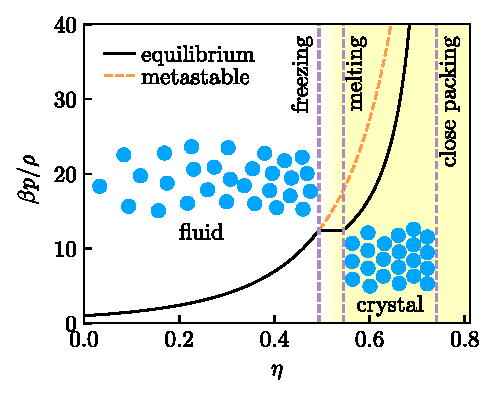
\includegraphics[width=0.75\linewidth,outer]{hs-phase-diagram}
  \caption[The hard sphere phase diagram]{
    The one-dimensional hard sphere phase diagram in terms of volume fraction, and its accompanying equation of state including the metastable branch.
    Equations of state adapted from Refs.\ \cite{CarnahanJCP1969,SpeedyJPCM1998,BannermanJCP2010}.
  }
  \label{fig:hs-phase-diagram}
\end{SCfigure}

\begin{SCfigure}
  \includegraphics[width=0.75\linewidth,outer]{ball-pit-horizontal}
  \caption[Random close packing in a ball pit]{
    Random close packing of hard spheres in a ball bit.
    Image by Peter Ong.}
  \label{fig:rcp}
\end{SCfigure}

As the most widely studied model interaction potential we know a lot about its equilibrium structure (phase diagram) in bulk and even inhomogeneous thanks to density functional theory \cite{?,?,?}.
However, its behaviour off-equilibrium at high densities is hotly debated.
The two biggest unresolved research topics for this subject:
\begin{itemize}
\item \emph{Nucleation}: given that above freezing the crystal ? Theoretically predicted nucleation rates from simulation studies differ by 12 orders of magnitudes from experiments, purported to be the second biggest disagreement between theory and experiment in all of science \cite{?}.
\item \emph{Metastable liquid}: if one could avoid crystallisation and equilibrate only over the liquid microstates, what would be the ultimate fate of the liquid?
  We will talk more about this in \ref{?}.
\end{itemize}

Metastable liquid.
Evantually this falls out of equilibrium.
In recent years a consensus has been forming.
We will return to talk more about glasses and the supercooled liquid this in section \ref{sec:glass} of the literature review.

We mention some other open problems of hard spheres, that will not be directly addressed though many of the ideas and methods developed in this thesis could transfer.
There is a deep connection between hard spheres and computer science.
Packing problems have been studied \cite{Cohn2016,Conway1999} and they are notoriously difficult; Kepler conjectured the optimal packing in 3d was the face-centred cubic/hexagonal close packing but it took 300(?check) years to solve this.
The final proof was computer aided, and not simple.
Packing problems are connected with encoding/encryption.
Transmitting a signal requires a way to encode a message across a band(?): if packed too tightly on the band(?) then noise will destroy the signal to it is desirable to optimise the sites for bits \cite{Cohn,?,?}.
Additionally, lattice based encryption techniques are one of the alternatives to prime factorisation: the coming development of quantum computers \cite{?,?} would render prime factorisation easy because of Shor's algorithm \cite{Shor?} rendering standard encryption techniques insecure.
The techniques developed for the mean field hard sphere problem have been applied to the perceptron model \cite{?}, and deep-learning neural networks which are naturally high dimensional problems lending themselves to a mean field treatment \cite{?}.

Hard spheres will be the focus of the first 3 chapters.
Although hard spheres will be our focus, we will mention the importance of systems of hard particles of other shapes for self-assembly.
We will indicate the route to doing this throughout, and we will do this explicitly in \ref{chapter:resummation}.
Self-assembly is an active area of soft matter: it is technologically desirable to tailor the final structure by controlling the building blocks.
Imagine assembling nanomachines or artificial cells by controlling the chemistry.
It is found that varying the size and shape of hard particles can reproduce all the complexity of the periodic table \cite{Glotzer?,Dijkstra?}.
Hard spheres are the simplest such system, so a theory which can treat other geometries is desirable.

Structure of thesis.

The primary goal of this thesis is to advance the methods of treating liquids at high densities, particularly concerning the role of thermodynamics in dynamical arrest and nucleation.
The problem that we solve is quite general: given an interaction potential, what kinds of structures form in the bulk liquid.
To the best of our knowledge this problem has not been solved for an atomistic interaction potential.
Admittedly the system we choose as simple as possible while still remaining physical, but it's a start.
One can imagine this method being useful in more complex systems such as protein folding in aqueous solution, predictive self-assembly of complex structures, predictive chemical reactions etc.

The liquids and glass community do not have a great deal of overlap.
The glass community , in spite of recent advances in liquids
However a small community of .
The aim of chapters will be to introduce these ideas into glassy physics.
In reflection of this, the literature review of \ref{chapter:background} will focus on methods of liquid state theory.
We will be advancing liquids into glasses, so while it is important that we review the paradigms of glassy physics, we will not be using methods developed intrinsically for glasses.

The method is entertaining and somewhat counterintuitive: a scheme to predict things about a macroscopic system from fewer particles than a person (traditionally) has fingers.

A secondary goal would be to advance the understanding of the fundamental theory of hard particles in some small way.
I have attempted to develop the geometrical theory behind the methods of Chapters \ref{chapter:morphometric-framework} and \ref{chapter:morphometric-applications} in a generally applicable way.

In chapter \ref{chapter:aerosols} we will change subject to the study of nucleation kinetics in drying aerosols.
This project emerged from an opportunity to collaborate with the Bristol Aerosol Research Centre, so it was driven by experimental conditions which are not adequately captured by a purely hard sphere model.
The nucleation theory we employ is identical to that used to describe hard sphere crystallisation, so the questions posed are fundamental despite the applied context.
We intended to keep this chapter self-contained, so we save full discussion of nucleation until chapter \ref{chapter:aerosols}.

\ifdefined\includebibliography
  \printbibliography
\fi
  
\end{document}
